
\def\raggedright{}
\documentclass[11pt]{beamer}

\usepackage[utf8]{inputenc}
\usepackage[francais]{babel}

\usepackage{ulem}

\usepackage{color}
\definecolor{brown}{rgb}{0.69,0.2,0.2}

\usecolortheme{mydolphin}
\useoutertheme{mysplit}
\useinnertheme{circles}

%\beamertemplateshadingbackground{blue!5}{red!5}

%\usetheme{Singapore}
%\usetheme{Darmstadt}
\usetheme{Lyon}



\title{The Discovery Project}
\author{{\small Cédric Tedeschi}}
\date{\small{\textcolor{gray}{September 10, 2013}}}

\mode<presentation>
\beamertemplatetransparentcovereddynamic

\usepackage{texgraphicx}
\usepackage{epsfig}
\usepackage{pgf,pgfarrows,pgfnodes,pgfautomata,pgfheaps}

\setbeamerfont{block title}{size={}}

\newcommand{\cframe}[1]{\frame[label=current]{#1}}

\setbeamertemplate{navigation symbols}{}

\begin{document}

\frame[plain]{

    \titlepage 
}

\frame{
  \frametitle{Next Generation Utility Computing ?}

\begin{columns}
  \begin{column}{.7\linewidth}
    \begin{block}{Current Trends}
      \begin{itemize}
      \item Data centers of ever-increasing size
      \item High energy consumption
      \item Find new (colder) locations ?
      \end{itemize}
    \end{block}
  \end{column}
  \begin{column}{.3\linewidth}
    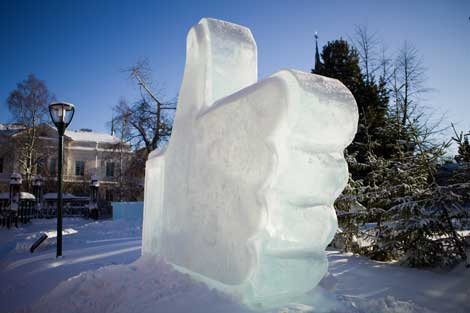
\includegraphics[width=\linewidth]{fig/like.jpg}
  \end{column}
\end{columns}
\pause
  \begin{alertblock}{But...}
    \begin{itemize}
    \item Legal issues
    \item Reliability limitations
    \item {\bf Long distance connections}
    \end{itemize}
  \end{alertblock}



}

\frame{
  \frametitle{Locality}

  \begin{exampleblock}{A use case for locality}
    \begin{itemize}
      \item Online ordering service
      \item Clients are locals
      \item Deployment in the 'ice cloud'?
        \begin{itemize}
          \item Extra energy consumed
          \item Increased latency
          \item Amount of network exchanges
        \end{itemize}
    \end{itemize}
  \end{exampleblock}

\pause
  \begin{alertblock}{}
    \begin{center}
      {\bf Need for alternative designs}
    \end{center}
  \end{alertblock}


}

\frame{
  \frametitle{Approaches}

  \begin{block}{Beyond the cloud?}
      \begin{itemize}
      \item Hybrid / Federated cloud ?
      \item Micro Data centers at the edge of the network ?
      \item Fog Computing ?
      \item (Seasonal) data furnaces
      \end{itemize}
    \end{block}
}

\frame{
  \frametitle{The Discovery Initiative}

  \begin{center}
    
\includegraphics[width=.3\linewidth]{fig/rocket.png}
  \end{center}
  \vspace{-.5cm}
    \begin{block}{Involvements}
      \begin{itemize}
        \item PI: Adrien Lèbre (Ascola)
        \item Asap, Avalon, Myriads
        \item Orange
        \item Renater
      \end{itemize}
    \end{block}

\begin{columns}
  \begin{column}{.33\linewidth}
    
\includegraphics[width=.9\linewidth]{fig/renater.png}
  \end{column}
  \begin{column}{.33\linewidth}
    
\includegraphics[width=.9\linewidth]{fig/inria.jpg}
  \end{column}
  \begin{column}{.33\linewidth}
    
\includegraphics[width=.9\linewidth]{fig/orange.png}
  \end{column}
\end{columns}
}


\frame{
  \frametitle{The Discovery Initiative (2)}
  \vspace{-2cm}
  \flushright{
\includegraphics[width=.2\linewidth]{fig/rocket.png}}
  \begin{itemize}
    \item One key idea: leverage the backbone's over-provisioning
      \begin{itemize}
      \item Power
      \item Cooling systems
      \item Routers
      \end{itemize}
    \item \emph{Room} for adding resources directly in the backbone
    \end{itemize}

}

\frame{
  \frametitle{The Renater Example}
  \begin{center}
  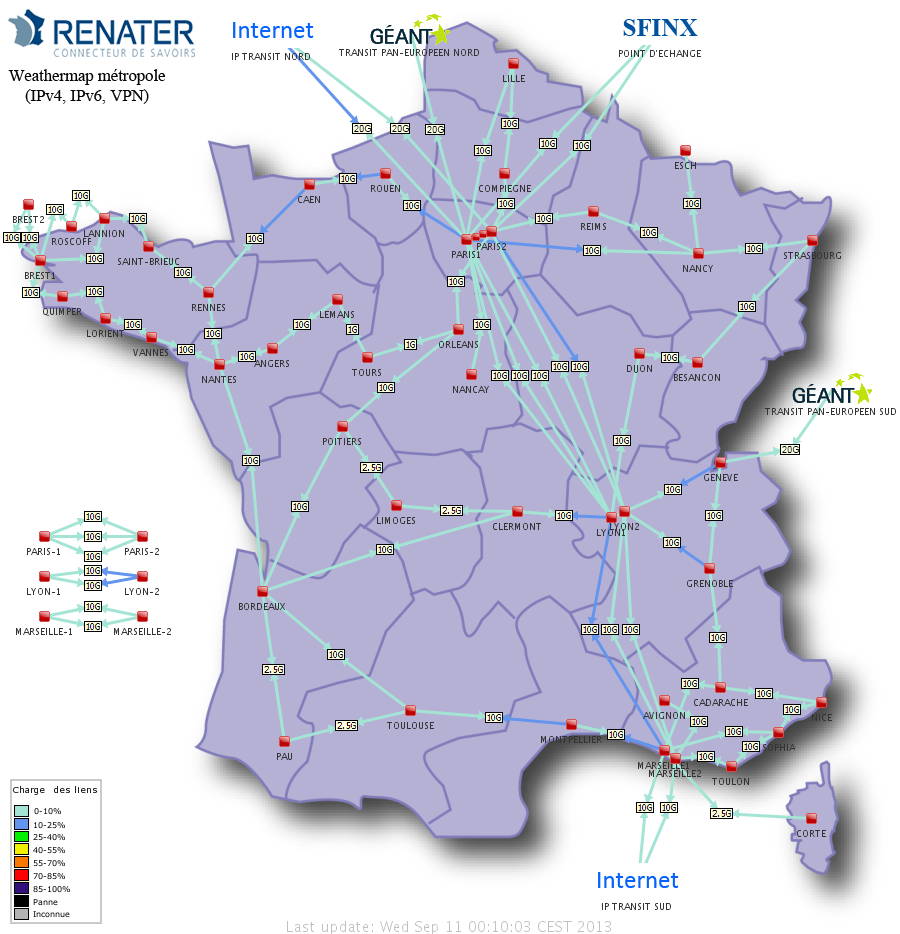
\includegraphics[width=.7\linewidth]{fig/renater_map.png}
  \end{center}
}

\frame{
  \frametitle{The Renater Example (2)}

  \vspace{-.5cm}
  \begin{flushright}
    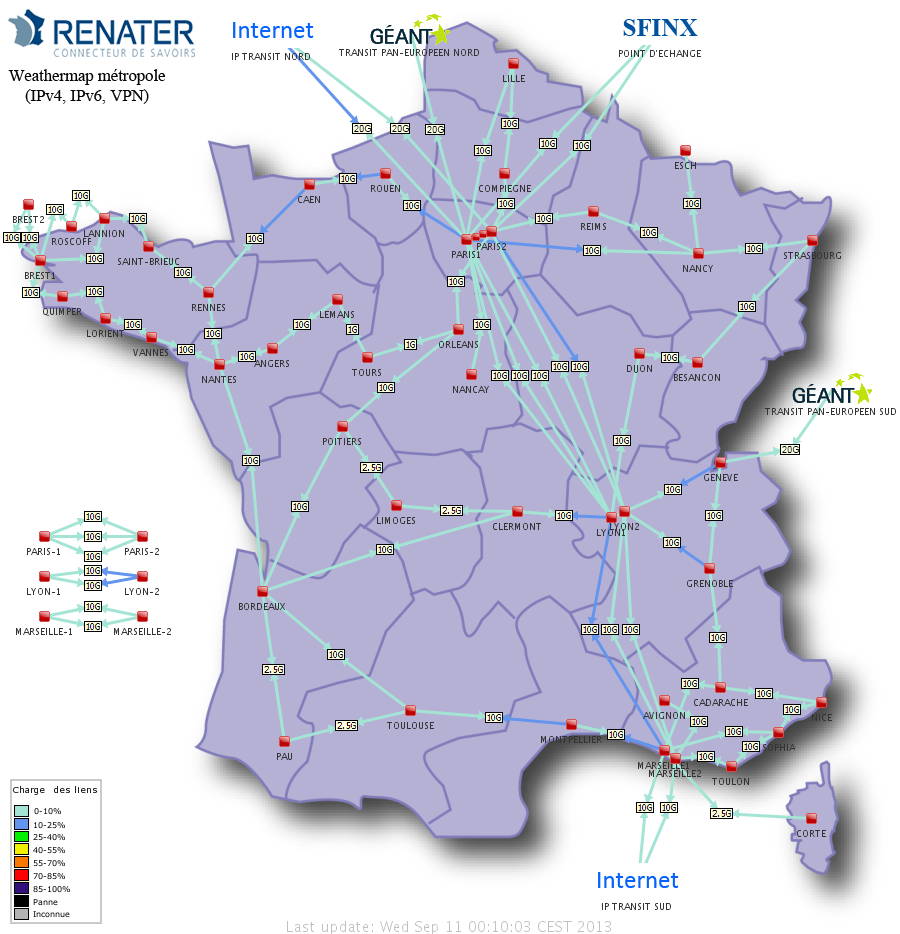
\includegraphics[width=.3\linewidth]{fig/renater_map.png}
  \end{flushright}

  \vspace{-2.5cm}
  \begin{itemize}
  \item Underutilised links 
  \item Shaped and renewed according to PoP
  \item Redundancy
  \end{itemize}

  \begin{block}{Vision}
    \begin{itemize}
      \item Deploy UC infrastructures tightly-coupled with the network
      \item Renater $\Rightarrow$ GEANT $\Rightarrow$ ...
      \item Ideally: leverage the routers' idle computing power
      \item Realistically: extend network hubs with servers 
        \begin{itemize}
        \item dedicated to VM hosting
        \item proportionally to the PoP size
        \end{itemize}
      \end{itemize}
    \end{block}

}

\frame{
  \frametitle{A Distributed Backbone-based Cloud}

  \begin{block}{}
    \begin{center}
    {\bf Distributed intra-backbone interconnected servers}
    \end{center}
  \end{block}

  \begin{block}{Single system}
    \begin{itemize}
    \item Overlay layer
    \item Find close adequate nodes
    \item Retrieve an object? (VM)?
    \item Deal with the scale and uncertainty
    \end{itemize}
  \end{block}


}

% \frame{

%   \begin{center}
%     {\huge Basic Usage ?}
%   \end{center}

% }

\frame{
  \frametitle{On-going work}

  \begin{itemize}
  \item Overlay definition
    \begin{itemize}
    \item Somewhere between a DHT and simple gossip
    \item Finding close nodes and routing
    \end{itemize}
  \item INRIA  RR 8348
  \item INRIA National Lab
  \end{itemize}

}

\end{document}



